
\documentclass[13pt,compress]{beamer}
% deactivate beamer navigation
%\setbeamertemplate{navigation symbols}{}
%\usepackage{geometry}
%\geometry{papersize={180mm, 135mm}, top=-1.5mm} % 210mm, 297mm

\usepackage[nospeakermargin]{../style/lmu-lecture}

\setbeamertemplate{frametitle}{\expandafter\uppercase\expandafter\insertframetitle}
%\useoutertheme{metropolis}
% remove section slides
\AtBeginSection[]
{
  \begin{frame}<beamer>
    \frametitle{Part 2}
    \tableofcontents[currentsection]
  \end{frame}
}
% includepdf slides, pagecommad will set counter for framenumber
\usepackage{pdfpages}
\includepdfset{trim=0mm 0mm 0mm 0mm, pagecommand={\global\setcounter{framenumber}{\value{page}}}}
% trim=0mm 6mm 0mm 0mm, offset=0 15,
% add footer:
\usepackage{framed, color}
\usepackage{xcolor}
%\iffalse
\setbeamertemplate{footline}[text line]{%
    \noindent\hspace*{\dimexpr-\oddsidemargin-1in\relax}%
     \colorbox{white}{
     \makebox[\dimexpr\paperwidth-2\fboxsep\relax]{
     \color{black}
     \begin{minipage}[c][4.5ex][c]{0.5\linewidth}
       \secname
     \end{minipage}
     \hfill\begin{minipage}[c][4.5ex][c]{0.5\linewidth}
       \flushright
       \insertframenumber{}~/~\inserttotalframenumber~~
     \end{minipage}
     }}%
  \hspace*{-\paperwidth}
}
%\fi

\title{Introduction to Machine Learning\\with R and mlr3}
\author{Bernd Bischl \& Marvin N. Wright}
%\institute{Essential Data Science Training}
\date{DAGStat, March 2025}



\begin{document}
\setbeamercolor{background canvas}{bg=}

% General remark: hyperlinks in included pdfs are not clickable anymore in the combined pdf

\frame{\titlepage}

\section{Resampling}
\includepdf[pages={7}, trim=0mm 0mm 45mm 0mm]{../slds-lecture-pdfs/lecture_i2ml/slides-pdf/slides-evaluation-generr.pdf}
\includepdf[pages={2, 7, 4-6, 8-9}, trim=0mm 0mm 45mm 0mm]{../slds-lecture-pdfs/lecture_i2ml/slides-pdf/slides-evaluation-resampling-1.pdf}
\includepdf[pages={12-14}, trim=0mm 0mm 45mm 0mm]{../slds-lecture-pdfs/lecture_i2ml/slides-pdf/slides-evaluation-test.pdf}
\includepdf[pages={2-4,8-10}, trim=0mm 0mm 45mm 0mm]{../slds-lecture-pdfs/lecture_i2ml/slides-pdf/slides-evaluation-resampling-2.pdf}
%\section{Resampling with mlr3}
%\includepdf[pages={3, 5, 8-9, 11, 13, 18-23, 27-31}]{../slds-lecture-pdfs/mlr-doc/CURRENT_mlr3_course/01_mlr3/mlr3-resampling.pdf}
%\section{Exercise: Resampling with mlr3}
%\begin{frame}{Exercise: Resampling with mlr3}
%File: \textit{day1\_resampling.html}
%\end{frame}
%\section{Benchmarking with mlr3}
%\includepdf[pages={33-36, 40-41, 43, 45-46, last}]{../slds-lecture-pdfs/mlr-doc/CURRENT_mlr3_course/01_mlr3/mlr3-resampling.pdf}
%\section{Exercise: Benchmarking with mlr3}
%\begin{frame}{Exercise: Benchmarking with mlr3}
%File: \textit{day1\_benchmarking.html}
%\end{frame}



\end{document}
